

\documentclass{article}
\usepackage{hyperref}
\usepackage[utf8]{inputenc}
\usepackage{graphicx}
\usepackage{listings}
\usepackage{xcolor}
\lstset { %
    language=C,
    backgroundcolor=\color{black!5}, % set backgroundcolor
    basicstyle=\footnotesize,% basic font setting
}
 
\begin{document}

\begin{titlepage}
	\centering
	\vspace{1cm}
	{\scshape\Large PAR Laboratory Assignment\par}
	\vspace{0.75cm}
	{\Large Course 2018/19 (Fall semester)\par}
	\vspace{0.75cm}
	{\huge\bfseries Lab 2:  Embarrassingly parallelism with OpenMP: Mandelbrot set\par}
	\vspace{1cm}
	{\Large\itshape Pablo Vizcaino, Guillem Ramírez\par}
    \vspace{0.5cm}
    {\Large User: Par2206\par}
    \vfill
% Bottom of the page
	{\large \today\par}
\end{titlepage}

 
\clearpage
\tableofcontents
\clearpage 

\section{Introduction}
\begin{flushleft}
In this laboratory we are going to study the task decomposition and the parallelization strategies of the computation of the Mandelbrot set.
\end{flushleft}

\begin{flushleft}
The Mandelbrot set is a set of complex numbers \textit{C} obtained from iterating the equation $Z = z^2 + C$.
You can see a visualization of the result from the computation in the figure \ref{fig:mandelbrot1}
\end{flushleft}

\begin{figure}[ht]
    \centering
    
\includegraphics[width=0.75\textwidth]{mandelbrot.jpg}
    \caption{Mandelbrot visualization}
    \label{fig:mandelbrot1}
\end{figure}
\newpage
\section{Parallelization strategies analysis}
\begin{flushleft}
Our first objective is to analyze the data dependency within the Mandelbrot computation. With this purpose we decided to explore row and point granularity. All executions with tareador use the option -w 8, which means 8 iterations per loop.
\end{flushleft}
\subsection{Point decomposition}
In this section we are presenting the point decomposition strategy , where we are creating at each inner loop iteration a task.
\subsubsection*{Point decomposition analysis with \textit{tareador}}
We just needed to add tareador start task directive in the beginning of the inner for loop and a tareador end task at the end of the inner for loop. You can find the source code at \textit{code/tareador/mandel-tar-point.c}. Listing \ref{code:tareadorPoint} shows the structure.

\begin{lstlisting}[caption={Tareador instrumentation at point granularity},label=code:tareadorPoint]
    /* Calculate points and save/display */
    for (row = 0; row < height; ++row) {
        for (col = 0; col < width; ++col) {
            tareador_start_task("point");
                        .
                        .
                        .
            tareador_end_task("point"); 
\end{lstlisting}

\begin{flushleft}
The result obtained from executing \textit{run-tareador.sh} with \textit{mandel-tar} objective (non-graphical version) is:
\end{flushleft}
\begin{figure}[ht]
    \centering
    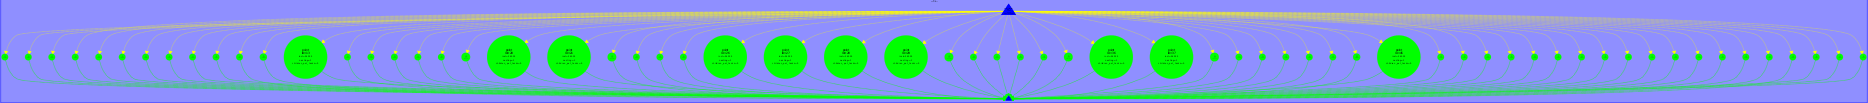
\includegraphics[width=1\textwidth]{mandel-tar-point-graph.png}
    \caption{Tareador graph with point granularity}
    \label{fig:tareadorpoint}
\end{figure}
\begin{flushleft}
From the graph obtained we can observe that there are 64 non-dependant tasks, one for each point: $64 == 8*8$. 
Due to the big number of tasks the graph is in a long shape, you can view the source image at \textit{img/tareador/mandel-tar-point-graph.png}. From the graph we can conclude that working with a big number of tasks can carry out to overheads. 
\end{flushleft}
\newpage
\subsection{Row decomposition}
In this section we are presenting the row decomposition strategy, where we are creating a task for each row of points. 
\subsubsection*{Row decomposition analysis with \textit{tareador}}
For this analysis we just need to add tareador directives in the middle of the for loops. You can find the source code at \textit{code/tareador/mandel-tar-row.c}. Listing \ref{code:tareadorRow} shows the structure.

\begin{lstlisting}[caption={Tareador instrumentation at row granularity},label=code:tareadorRow]
    /* Calculate points and save/display */
    for (row = 0; row < height; ++row) {
        tareador_start_task("row");
        for (col = 0; col < width; ++col) {
                    .
                    .
                    .
        }
        tareador_end_task("row");       
    }
\end{lstlisting}
\begin{flushleft}
The result from executing \textit{run-tareador.sh} with \textit{mandel-tar} objective (non-graphical version) is:
\end{flushleft}
\begin{figure}[ht]
    \centering
    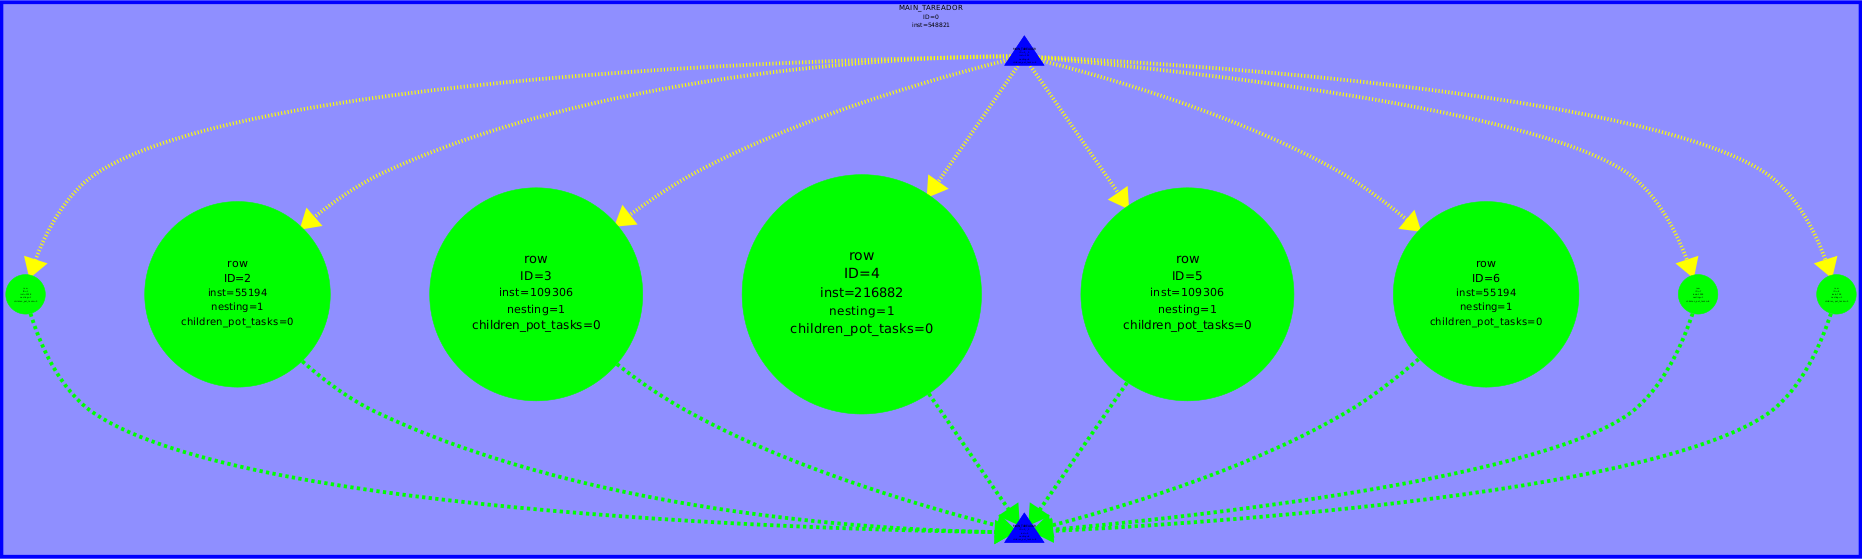
\includegraphics[width=0.99\textwidth]{mandel-tar-row-graph.png}
    \caption{Tareador graph with row granularity}
    \label{fig:tareadorrow}
\end{figure}

\begin{flushleft}
From the graph we can observe that we get 8 non-dependant tasks, one for each row, as expected. With less tasks we may have less overheads from the previous version but we may not be taking profit of all threads. This question will be evaluated in the following sections. The source image is at \textit{img/tareador/mandel-tar-row-graph.png}. 
\end{flushleft}
\newpage
\subsection{Preliminary comparison between strategies}
\begin{flushleft}
After analyzing the two versions we find out that with a point based strategy the number of tasks is: $w^2$ . In our case w is 8 so the number of tasks is 64, this number can increase to really high values in default executions and can be really problematic due to task creation and work distribution overheads. In the other hand we find out that row granularity the number of task linearly increase with w, which may be a more affordable value. This general guidelines and ideas will be taken into account for the next sections.
\end{flushleft}
\subsection{Graphical version analysis}
\label{sec:graphical}
\begin{flushleft}
Once the granularity of the computation itself is evaluated, we will be analyzing the graphical version. For this purpose we will be using the same source code as in the previous subsection (\textit{code/tareador/mandel-tar-row.c}) but we will be compiling using the \textit{mandeld-tar} Makefile target. 
\end{flushleft}

\begin{figure}[ht]
    \centering
    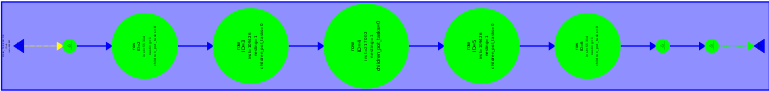
\includegraphics[width=0.99\textwidth]{r-mandeld.png}
    \caption{Tareador graph with mandeld target}
    \label{fig:tareadormandeld}
\end{figure}

\begin{flushleft}
The image is rotated for document structuring purpose. The full non-rotated image can be found in \textit{img/tareador/mandeld-tar.png}.
\end{flushleft}
\begin{flushleft}
We can observe that due to dependencies the graph is now serialized, if we look into the edges between tasks in tareador we can see that a graphics library variable is now needed between iterations. This is causing the serialization of the graph.
\end{flushleft}
\begin{figure}[h]
    \centering
    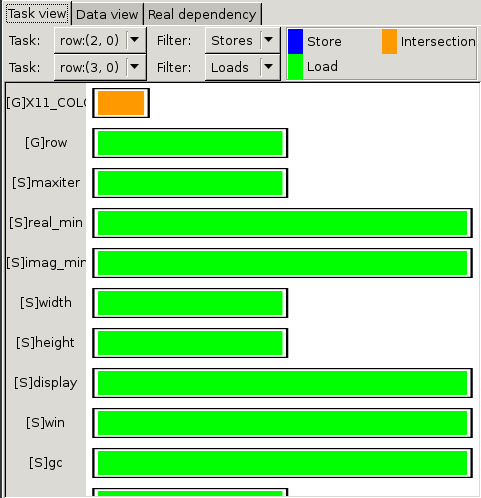
\includegraphics[width=0.32\textwidth]{mandeld-tar-edge.png}
    \caption{Variable usage between tasks}
    \label{fig:mandeldtaredge}
\end{figure}
\begin{flushleft}
If we look into the code we can find that the the part causing serialization of the task graph is:
\end{flushleft}
\begin{lstlisting}
    #if _DISPLAY_
            /* Scale color and display point  */
            long color = (long) ((k-1) * scale_color) + min_color;
            if (setup_return == EXIT_SUCCESS) {
                XSetForeground (display, gc, color);
                XDrawPoint (display, win, gc, col, row);
            }
    #else
\end{lstlisting}
\begin{flushleft}
Specially what is causing serialization is the inner if statement. In the following sections we will be parallelizing the code, for protecting this part we will be adding the following clause before the if statement so that we are telling openMP that only one thread can be working at any time.
\end{flushleft}
\begin{lstlisting}
    #pragman omp critical
    if (setup_return == EXIT_SUCCESS) {
\end{lstlisting}
\newpage
\section{Parallelization strategies implementation}
In this section we are going to present the implementation of both strategies in \textit{OpenMP}
\subsection{Point decomposition in \textit{OpenMP}}
For this strategy we went through a few versions. Starting with the initial version and making improvements.
\subsubsection*{Initial version}
The initial version was given in the assignment and its:
\begin{lstlisting}
    for (row = 0; row < height; ++row) {
        #pragma omp parallel
        #pragma omp single
        for (col = 0; col < width; ++col) {
            #pragma omp task firstprivate(col)

\end{lstlisting}
\begin{flushleft}
In this version we introduced the firsprivate pragma which tells the compiler that the col variable inside the construct is a new variable initialized to the same original variable value.
\end{flushleft}
\begin{flushleft}
Also notate that in the full code \textit{code/omp/mandel-omp-initial.c} we added the \textit{\#pragma omp critical} clause in the region that generated dependencies, see: \hyperref[sec:graphical]{\textit{graphical version analysis}}.
\end{flushleft}

\begin{figure}[h]
    \centering
    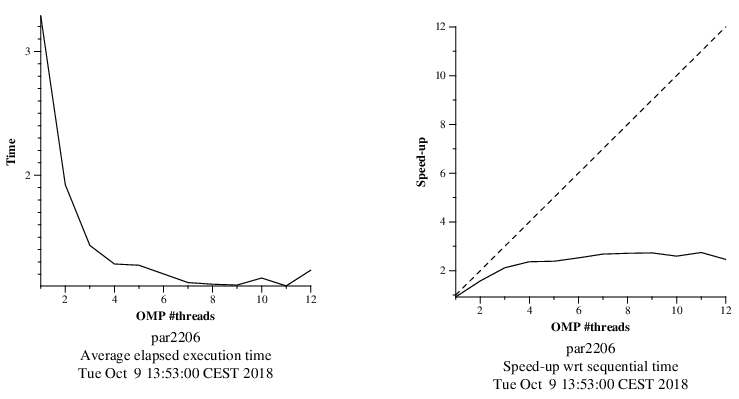
\includegraphics[width=1\textwidth]{strongPoint.png}
    \caption{Strong scalability plots for initial version}
    \label{fig:strongpoint}
\end{figure}
\begin{flushleft}
We can observe that the speedup poorly improves with the increase of \#threads that's due to the version not being optimized as we create a lot of tasks and the work distribution takes into serious overheads.
\end{flushleft}
\section{Performance comparison}
\section{Conclusions}

\end{document}

